% !TEX TS-program = pdflatex
% !TEX encoding = UTF-8 Unicode

\documentclass[preprint]{sigplanconf}

\usepackage{graphicx,listings,fixltx2e}

\begin{document}
\conferenceinfo{PLDI 2011}{June 4--8, 2011, San Jose, CA, USA.}
\copyrightyear{2010}

\preprintfooter{PLDI 2011}
\titlebanner{DRAFT---Do not distribute}

\title{Parakeet: An Array-Based Framework for High-Level GPGPU Programming}
%\authorinfo{Anonymous}

\maketitle

\begin{abstract}
GPUs are now often being used as general-purpose accelerators, since they have
far greater memory bandwith and processor count per dollar and per watt than
contemporary CPUs.  However, the current tools, such as CUDA and OpenCL,
available for programming GPUs are cumbersome and very low level, thus forcing
a tradeoff between programmer productivity and program performance.

In orderWe present Parakeet, a dynamic runtime/JIT compiler for high level,
dynamic array languages that targets NVIDIA GPUs.

for Q,  a high-level array
language of the APL family, which targets NVIDIA GPUs. Q is a highly dynamic
language with a rich set of
array operators and is well suited for rapid prototyping. The extensive use of
array operators in Q programs organizes a program's parallelism in such a way
that allows us to parallelize automatically and transparently
many computational kernels while avoiding the common pitfalls
associated with the analysis of loops. Our optimization techniques allow Q
implementations of two benchmark problems to achieve speeds within a
factor of XX of hand-coded GPU programs for those problems.
\end{abstract}

\section{Introduction}

Parallelism has become ubiquitous in modern processors, with all major CPU
manufacturers increasing processor performance by adding more and more cores as
opposed to boosting processor clock speeds \cite{Asan06}.  In addition to the
move to multicore CPUs, the massive increase in performance
of modern GPUs and the development of frameworks for doing general-purpose
programming on them has led to much recent interest in general-purpose GPU
programming (GPGPU) as a way to speed up various computational workloads. While
with the advent of frameworks such as OpenCL \cite{Muns10} and NVIDIA's CUDA
\cite{NvidCU}, GPGPU programming has gotten somewhat easier, it is still much
more difficult than traditional sequential programming, requiring much
domain-specific and architectural knowledge.

% The following paragraph was inspired by, and is perhaps too similar to, the
% same paragraph from the Copperhead intro
As a step toward making GPGPU and multicore programming easier for the
programmer, we focus on enabling high level expression of data parallel
programs. Nested data parallelism, as described by Guy Blelloch in his work on
NESL \cite{Blel90}, captures the potential parallelism in many important
algorithms and problems, such as linear algebra and many machine learning
algorithms.  In addition, data parallel programs map well to modern
parallel processor hardware. For example, modern Intel processors offer 8- and
16-wide vector operations, while modern GPUs execute instructions on 32- or
64-wide SIMD arrays of coupled processors. Thus, the substantial
performance potential of these processors is naturally tapped by data
parallelism.

In this spirit, we present a parallelizing dynamic runtime/JIT compiler for
high level array languages.  Array languages, such as those from the APL family
[INSERT CITE] or a data parallel subset of Matlab [INSERT CITE], are well suited
to expressing nested data parallel computations. In our system, programmers
write code in a dynamic high level language with native array types and array
operators. These array operators embody many standard data parallel primitive
operations--such as Map, Reduce, and Scan--in a lightweight, natural way.  Our
runtime identifies sections of code that can potentially be parallelized and
run on the GPU.  These sections are translated to our high level data parallel
intermediate language, and undergo a series of optimizations including fusion
of data parallel operators.  The code is then compiled to parallel GPU
implementations and run on GPUs.

We view our techniques as largely language-agnostic so long as the input
language in question supports our data parallel primitives, but to build a
complete system we had to start with some given language and some back end
architecture target.  We chose to implement our first front end for Q, a
sequential array language from the APL family developed by Kx Systems that is
heavily used in financial computing \cite{Borr08}.  Our first back end currently
targets NVIDIA GPUs by emitting code in PTX, NVIDIA's GPU pseudoassembly
language.  We are currently working on another front end for a data parallel
subset of Matlab.

The main contributions of this paper are the following:

\begin{itemize}
\item We present a codification of an automatic parallelization process for
high level data parallel programs.
\item We present a series of compiler optimizations for our intermediate data
parallel language, and some dynamic runtime tuning procedures that greatly
improve the overall performance of the system.
\item We evaluate our framework on a pair of standard benchmark programs, and
show that our system is able to deliver competitive performance as compared
with tuned CPU and GPU implementations.
\end{itemize}

\section{Q: A High-Level Array Language}
\label{Q}

Q is a high-level, sequential array programming language from the APL family.  Q is dynamically typed, and the standard proprietary implementation is interpreted as opposed to compiled.  Q is a fully-featured language, including such things as functions for reading and parsing comma-separated-value input files, performing I/O, and a SQL-like query language for querying its built-in in-memory database.  Further, Q has many built-in operators for manipulating arrays, and comes with a set of {\it adverbs}, which are second-order function modifiers that are used to apply functions to all elements of $n$-dimensional arrays.  Thus Q provides a convenient environment for rapidly prototyping large-data computations, and this has led to its widespread adoption in the financial computing community.

\subsection{Examples}
\begin{figure}
\begin{verbatim}
1  f: {[x] 5 + 3 * x}
2  
3  / generate 100000-element random array
4  a: 100000 ? 10
5  b: f[6]
6  c: f[a]
\end{verbatim}
\caption{Q Mapping Example}
\label{QMap}
\end{figure}

\begin{figure}
\begin{verbatim}
1  sqr: {[x] x*x}
2  dist: {[x;y] sqrt sum sqr x - y}
3  
4  a: (1000;1000) # (1000000 ? 10)
5  b: (1000;1000) # (1000000 ? 10)
6  
7  all_dists: dist/:\:[a;b]
\end{verbatim}
\caption{Q All-Pairs Distance Example}
\label{QAllPairsDist}
\end{figure}

Figure \ref{QMap} gives an example of a simple Q program.  In line 1, we define a function \texttt{f} which takes a single argument \texttt{x} and computes a simple linear function of it.  In Q syntax, the colon operator is used for assignment, and curly braces surround function definitions.  Brackets are used to declare function arguments, with semicolons serving as list delimiters between the various arguments.  Q functions return the result of their final statement; there is no \texttt{return}-like keyword as in C-like languages.  On line 3 we see a comment, denoted by a single \texttt{/}, and on line 4 we use the \texttt{?} random number generation operator to generate a 100000-element array of integers between 0 and 9.

In line 5, we finally perform our first computation, evaluating \texttt{f} on the input 6 with the bracket syntax, and storing the value 23 in variable \texttt{b}.  Line 6 evaluates \texttt{f} element-wise on the entire array \texttt{a}, storing the result in \texttt{c}.

This code snippet illustrates a key feature of Q for our purposes.  Functions are agnostic to the shape of their input arguments--as we saw, \texttt{f} was legally applied both to a scalar input as well as an array.  In effect, the function \texttt{f} was {\it mapped} over the array \texttt{a}.  Thus we see that Q programs can express data-parallel computations both very compactly, and in a declarative, high-level fashion.  No explicit looping over the elements of \texttt{a} is required.

In Figure \ref{QAllPairsDist}, we see a slightly more complicated example.  First we define a pair of functions--one which computes the square of an input variable, and another which computes the Euclidean distance of two input vectors.  The \texttt{sum} function is a built-in {\it reduction} function, which computes the sum of all elements of its input argument.  Q has many such built-in functions.  Next, we generate two 1000x1000 random matrices.  The \texttt{\#} operator is used to modify the shape of a variable: its left argument is a list of lengths for the dimensions, and the right argument is a variable whose shape is to be modified.  The above code generates two one-million-element random 1-dimensional arrays and then reshapes them to be square 2-D matrices.  The parenthesis syntax with semicolons as delimiters is used to declare lists.

Finally, we evaluate the \texttt{dist} function on the matrices \texttt{a} and \texttt{b}.  In order to perform the computation we desire, viz. computing the pairwise distance between each row of \texttt{a} and each row of \texttt{b}, we use a new construct: {\it adverbs}.  In Q, adverbs are second-order function modifiers which are placed immediately after a function in its invocation.  They modify the behavior of the function in various ways.  In this case, we place the {\it each-right} and {\it each-left} adverbs after the call to \texttt{dist}.  (Their syntactic representations are \texttt{/:} and \texttt{\textbackslash:} respectively.)  Without these adverbs, the call to \texttt{dist[a;b]} would still be legal, but Q would map the \texttt{dist} function over the rows of \texttt{a} and \texttt{b} one-by-one, pairing up the first row of \texttt{a} with the first row of \texttt{b}, then the second row of each with each other, and so on.  The result would be a 1000-element vector of distances, as opposed to the 1000000-element matrix of all pairwise distances that we desire.

The each-right adverb modifies the call to \texttt{dist} so that it pairs the entire first argument to the function with each element of the second argument.  Thus, if one were to call the function \texttt{dist/:[a;b]}, this would produce a 1000x1000 matrix, where row \texttt{i} holds the result of computing \texttt{dist[a;b[i]]}.  This illustrates another point about Q: in the legal function call \texttt{dist[a;b[0]]}, the first argument is a 2-D matrix (in reality, a list of lists), while the right argument is a 1-D list.  Q automatically converts this call into a map, and logically expands the list \texttt{b[0]} into a matrix where each row is equal to \texttt{b[0]}.  It then computes the map of \texttt{dist}, with the result being a list of differences between like-numbered rows of the two matrices, just as in the case when we call \texttt{dist[a;b]}.

In order to get our desired result of an all-pairs-distances computation between the rows of \texttt{a} and \texttt{b}, we pair the each-right adverb with its mirror, each-left.  This combination, which is a common idiom in Q programming, can be used to produce Cartesian-product type computations, as it in turn applies the function to each pair of elements from both input arguments.

To emphasize the semantic compactness achievable with Q, compare the code listing in Figure \ref{QAllPairsDist} with the C version given in Figure \ref{CAllPairs}.  In order to express what can be captured in 3 lines of Q code, we need on the order of 20 lines of C, and the C given isn't even the most efficient possible (it doesn't include SSE vector instructions for example, which greatly increase the complexity of the code).  Arguably, the Q code is also much more readable once one gets used to Q's syntax.

\subsection{Q As a Skeletal Programming Language}
Q's adverbs and array operators form the subset of the language in which we are mainly interested: that which we can parallelize and map on GPUs.  The adverbs, given in Figure \ref{QAdverbs}, built-in functions such as the reduction \texttt{sum} we saw earlier, and the implicit mapping of functions over arrays form the basis of our skeleton-like parallel programming language.  Algorithmic skeletons \cite{Cole04} are a high-level parallel programming model which hide the complexity of synchronization and scheduling from the programmer by providing an interface of common parallel patterns such as Master-Slave, Map, and Reduce.

\begin{figure}
\centering
\begin{tabular}{|l|l|l|}
\hline Symbol & Name & Skeleton\\
\hline ' & each both & Map \\
\hline each & each monadic & Map \\
\hline /: & each right & Map \\
\hline \textbackslash: & each left & Map\\
\hline / & over & Reduce \\
\hline \textbackslash & scan & Scan \\
\hline ': & each previous & Map \\
\hline /:\textbackslash: & each left-each right & AllPairs \\
\hline
\end{tabular}
\caption{Q Adverbs}
\label{QAdverbs}
\end{figure}

The each Q adverbs should largely be self-explanatory: they all modify functions to apply elementwise to list inputs as opposed to being applied to the entire list directly.  For example, each-both is used to modify functions, such as the list concatenation operator, to apply pairwise to the elements of the input lists instead.

Within our compiler, we represent parallel computations by the following skeletons: Map, Reduce, Scan, and AllPairs.  Each of these higher-order skeleton functions takes as input another function (possibly another skeleton function) and that function's arguments.  In a sense, AllPairs is just a specific type of Map.  However, AllPairs computations generally result in repeated accesses to the same input data to generate many output results.  Thus they benefit from certain types of optimizations such as tiling, and in order to perform these optimizations we represent them as a separate skeleton.

Let us now see an example of how the two pieces of Q code above map to our internal skeletal representation.  In the Map case in Figure \ref{QMap}, the call to \texttt{f[a]} would simply be represented by the following skeletal pseudocode:

\begin{verbatim}
Map1([a], f)
\end{verbatim}

We choose to mark the cardinality of the skeletons, and to write the function arguments before the function itself.  This helps readability when the skeletons take nested skeletons as their functions.

In the all-pairs-distance case, we have a slightly more complicated scenario.  The \texttt{dist} function is modified by an AllPairs skeleton, but the \texttt{dist} function itself has both embedded Maps (the calls to \texttt{sqr} and \texttt{-}) and an embedded Reduce (the call to \texttt{sum}).  Thus the pseudocode for the direct translation of the Q to our skeletal representation is as follows:

\begin{verbatim}
AllPairs([as;bs],
  sqrt(Reduce1([Map1([Map2([a;b], -)], sqr)], +)))
\end{verbatim}

In this example, we see that skeletons can embed each other as well as sequential functions, and 

\section{CUDA Programming}
\label{GPU}

In this section we give an overview of modern GPU architecture (specifically, the NVIDIA GT200 architecture which we use in our evaluation) and the CUDA programming model.  Modern graphics processors are made up of arrays of simple shader processors, and when performing graphics computations these processors execute shader programs for performing rendering tasks.  With the advent of CUDA and other GPGPU programming environments such as OpenCL \cite{Muns08}, programmers can execute general-purpose programs directly on these processors as well.  For workloads amenable to streaming, data-parallel processing, GPUs can give orders of magnitude performance improvement over general-purpose CPUs.

In CUDA, a program is organized into {\it kernels}, which are sequential code run across many threads on the GPU's, or {\it device}'s, processors; and {\it host} code, which is the code run on the CPU.  Typically, a host thread launches a kernel onto the GPU, waits for results, and then launches further kernels.

A CUDA kernel's threads are organized into {\it thread blocks}, which are groups of threads that can communicate and share local resources.  Threads within a block can perform barrier synchronizations with each other via a CUDA intrinsic, but threads across blocks have no way to perform synchronization.  Thus, global synchronization among all threads in a kernel requires the program to be broken up into multiple kernel launches.  When launching a kernel, the programmer specifies how many thread blocks are required and how many threads to launch per block.  The standard idiom is for each thread to be assigned a small computation to be performed on a small subset of some large input data set.  The threads each are assigned a unique index which is used to determine the data for which they are responsible.

\begin{figure}
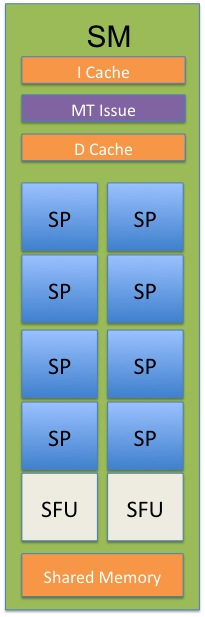
\includegraphics[height=80mm]{GPUdiagram1.jpg}
\caption{GT200 Architecture}
\label{GPUdiagram}
\end{figure}

The device's processors, shown in Figure \ref{GPUdiagram}, are grouped hierarchically, with each level of the hierarchy sharing certain hardware resources.  At the lowest level are symmetric processors or SPs, which are very simple sequential shader processors.  At the next level are symmetric multiprocessors or SMs, which are groups of 8 SPs that share an instruction issue and decode unit.  This means that all SPs within an SM execute their instructions in lockstep.  In the CUDA model, thread blocks are scheduled to run in their entirety on a single SM.  The SPs are then grouped to share texture processing units, and then these groups along with L2 caches make up the GPU chip.  The graphics card bundles the GPU along with a large block of off-chip DRAM, typically on the order of a few gigabytes in modern cards.

The CUDA model is a Single Instruction Multiple Thread or SIMT model, meaning that multiple threads with a block each execute the same instruction at the same time.  This differs from SIMD models in that branching instructions are allowed which diverge with a thread block.  However, this results in a significant performance degradation, as all threads in the block are then forced to execute both paths of the branch, with logical noops being executed by the threads on the path which didn't satisfy their conditional test.

In order to get maximum performance on a GPU, it is very important to manage memory usage.  While the peak memory bandwidth on modern GPUs is up to 150GB/sec or more--up to an order of magnitude higher than that of CPUs--this bandwidth can only be reached with careful access patterns on the part of threads within a block.  In addition, each SM has a 16KB scratchpad called {\it shared memory}.  The programmer must explicitly manage shared memory, and careful usage of it can result in orders of magnitude performance improvements over naively-written CUDA programs.  In addition, data must be manually moved between system RAM and the graphics card's DRAM.  Modern GPUs use PCI-Express, which has a maximum transfer rate of around 4GB/sec, which can easily become the major bottleneck in CUDA programs if memory transfers aren't managed carefully.

Various constraints limit how a programmer can structure his or her CUDA programs.  Each SM is able to execute a maximum of 8 thread blocks and a maximum of 1024 threads at a time.  In addition, a group of thread blocks can be co-scheduled on an SM only if they consume at most 16K registers, as each SM shares a register pool.  Finally, no more than 16KB of shared memory per SM can be used at a time, and so thread blocks with in aggregate exceed this limit cannot be co-scheduled.

\section{Compilation}
\label{Compilation}

As mentioned, our focus is on translating the data-parallel subset of the Q language into GPU kernels.  As such, our compiler is implemented as a plugin library to the extant Q interpreter.  We first preprocess Q modules, rewriting potentially parallelizable functions to call into our JIT compiler.  The programs are then run using the standard interpreter, and when such a rewritten function is executed, our JIT takes the datatypes of the arguments and compiles a GPU kernel (if one is not already present in the code cache).  Whenever the compiler is unable to compile a function or decides the overhead isn't worth it for whatever reason (such as data sizes being small), the compiler returns a message to the Q interpreter telling it to execute the original version of the function.  In this way, we are able to execute all Q programs in a manner transparent to the programmer other than running the preprocessor, while focusing our effort on the research questions related to high-level GPGPU programming.

We now give an description of our compilation steps in more detail.

\subsection{Preprocessing to Identify Parallelizable Functions}
We require that the Q programs we compile be self-contained modules.  This allows us to be certain that functions which do not perform I/O or write to global variables are side-effect free, which is a necessary property of GPU kernels since the graphics card is also unable to access RAM or I/O devices directly.  The programmer runs our preprocessor on his or her Q module, which parses the Q code and identifies functions which are functional and thus potentially parallelizable.  The preprocessor verifies that the transitive closure of all functions called by a given function $f$ satisfy the following constraints:

\begin{itemize}
\item No calls to ``unsafe'' functions which perform I/O operations.
\item No writes to non-local variables (global variables or variables outside the current scope).
\item Arguments to a parallel function called from a non-parallel function contain only data and no functions.  However, function values and higher-order functions are allowed.
\end{itemize}

Functions which only read global variables are allowed, and the preprocessor simply transforms global variable reads into explicit function parameters to the rewritten versions of the functions.  These constraints encourage a programming style where all the I/O and stateful computations are done in an outer unsafe layer of code, which then calls into a mostly pure (except for local state) chain of functions.  The output of the preprocessor is a new Q module which the programmer can then run in the normal way, and which the programmer never need modify directly.

\subsection{Data Flattening and Runtime Function Specialization}
At runtime, when the Q interpreter encounters a rewritten function this results in a call to our compiler runtime.  The compiler receives the data types of all the arguments as well as their sizes and looks up whether a compiled version of the given function for the given types exists in its compiled code cache.  If not, and the compiler decides that the data sizes warrant GPU execution of the function, it attempts to compile a GPU version of the function.  At this stage, the compilation is to a typed imperative intermediate language.  Otherwise, control is returned to the Q interpreter which then executes the original serial version of the function.

When a function is to be executed on the GPU, the input arguments must first be copied to the graphics card's DRAM.  Since the two memories don't share an address space, all pointer-based data structures must be flattened into a contiguous data layout prior to being copied.  The Q interpreter stores multi-dimensional arrays as lists of pointers to one-dimensional arrays, and so all such data structures must be flattened by the JIT compiler.  The compiler also maintains a directory of where the current version of a variable is currently stored--the CPU, the GPU, or both.  Data is only moved between the CPU and GPU when required, preventing unnecessary memory copies.

\subsection{Conversion to Dataflow Graph}


\subsection{Adverb Fusion and Other Optimizations}


\subsection{Evaluation of Dataflow Graph Triggers Kernel Compilation and Launch}
Once the final optimized dataflow graph has been generated, a runtime evaluator evaluates nodes in the graph whenever their input arguments are available.  When the evaluator encounters an adverb node such as an All-Pairs, it compiles this node into one or more GPU kernels, with different threads in the kernel assigned to different data elements in the computation.  Then, the input arguments which aren't already on the GPU are flattened and copied to the graphics card, and then the kernel is launched.

Various details complicate the above procedure.  First, imperative constructs such as a \texttt{for}-style loop can either be execute on the host by the evaluator itself, or they can be compiled to form part of the body of a kernel.  Which is better depends on many factors, and as of now we have simple heuristics in place for choosing.  We plan to explore optimizations in this sphere at a later point.

Second, certain primitives cannot be implemented by a single kernel launch.  An example is the parallel prefix sum algorithm of Blelloch \cite{Blel90}, which requires global synchronization between each of its recursive steps.  Since the only global synchronization mechanism available to a kernel is simply the termination of the kernel, such an algorithm must be implemented by multiple kernel launches.  Another example of an efficient parallel algorithm which requires global synchronization is the stream compaction algorithm of \cite{Bill09}.  The evaluator decomposes such dataflow graph nodes into the multiple kernels necessary to execute them, and launches them in the proper order.

\subsection{Runtime Tiling}
As mentioned, good use of shared memory is critical to achieving optimal performance of CUDA kernels.  One such use of shared memory is as a software-controlled cache of the graphics card's global DRAM.  A standard optimization in sequential programs is loop tiling, which involves setting the loop strides of nested loops such as to maximize data reuse of data resident in a CPU's caches \cite{Wolf91}.  A similar optimization on the use of shared memory as a cache is often extremely beneficial in the GPU domain.

In an All-Pairs computation, e.g.\ matrix-matrix multiplication, each input data element is involved in the computation of many output elements.  Thus, a naive implementation of the computation which directly accesses global memory whenever a particular input element is involved in a computation is extremely wasteful of memory bandwidth.  Instead, it is much better to cache some subset of the inputs in shared memory, compute as much as possible of the output from the data in shared memory, and then iterate this process by filling shared memory with a new subset of the input.

Our compiler generates GPU kernels which access data in this tiled fashion for All-Pairs computations.  The sizes of the tile windows of each input are determined based on the size of shared memory on the particular GPU and the sizes of each of the input elements.  Our evaluation shows this optimization to be extremely beneficial to performance.

\subsection{Example Output}

\begin{figure}
\begin{verbatim}
#include <math.h>
float dist(float *x, float *y, int len) {
  float sum = 0.0f;
  int i;
  for (i=0;i<len;++i) {
    sum += (x[i]-y[i])*(x[i]-y[i]);
  }
  return sqrt(sum);
}
void allpairs_dist(float *out, int vec_len,
                   float *xs, int num_xs,
                   float *ys, int num_ys) {
  int i,j;
  for (i=0;i<num_xs;++i) {
    for (j=0;j<num_ys;++j) {
      out[i*num_ys+j]=
        dist(xs+vec_len*i, ys+vec_len*j);
    }
  }
}
\end{verbatim}
\caption{C All-Pairs Distance Code}
\label{CAllPairs}
%\end{minipage}
\end{figure}

\begin{figure}
%\begin{minipage}{0.5\linewidth}
\begin{verbatim}
sqr:{[x] x*x}
dist:{[x;y] sqrt sum sqr x - y}
allpairs_dist:{[xs;ys] xs dist/:\: ys}
\end{verbatim}
\caption{Q All-Pairs Distance Code}
\label{QAllPairs}
%\end{minipage}
%\begin{minipage}{0.5\linewidth}
\end{figure}

\begin{figure}
%\begin{minipage}{0.333\linewidth}
\begin{verbatim}
__global__ void allpairs_kernel(
  float *out, int vec_len,
  float *xs, int num_xs, float *ys, int num_ys) {
}
\end{verbatim}
\caption{CUDA All-Pairs Compiled Output}
\label{CUDAAllPairs}
%\end{minipage}
\end{figure}

In this section we show an example output of our compiler on a simple All-Pairs kernel which we use as one of our benchmarks in Section \ref{Evaluation}.  The kernel computes the Euclidean distance between all pairs of vectors from two input lists of vectors.  The Q version is shown in Figure \ref{QAllPairs}.


\section{Evaluation}
\label{Evaluation}

We evaluated our compiler's performance on two benchmark programs: a Black-Scholes implementation which we translated to Q from the version includes in the PARSEC \cite{Bien08} benchmark suite; and a hand-written All-Pairs-Distance kernel based on that found in the K-Means Clustering implementation in the STAMP benchmark suite \cite{Minh08}.  For each benchmark, we generated performance results for each of the following implementations:

\begin{itemize}
\item The Q interpreter running the original Q code
\item A tuned CPU version written in C
\item A hand-written, tuned CUDA version
\item Our compiler's GPU version, with all optimizations turned off
\item Our compiler's GPU version with optimizations
\end{itemize}

Our experimental setup is as follows.  We ran our programs on a 4-core, 8-way hardware multithreaded Intel Xeon W3520 desktop machine with a 2.66GHz clock rate.  The machine has X GB of RAM, with a peak memory bandwidth of Y GB/sec.  The peak throughput of the CPU is U.UU GFLOP/s.

The GPU we used is an NVIDIA GTX280, which has 30 SMs and thus a total of 240 symmetric processors, each running at Y.YY GHz.  The card has D GB of global RAM, with a peak memory bandwidth of Y.YY GB/sec, and has a beak multiply-add throughput of U.UU GFLOP/s.

\section{Related Work}
\label{RelatedWork}

There's Copperhead \cite{Cata10}.  They're almost as good as we are.

There has been much recent work dedicated to making parallel programming easier.
The various approaches to addressing this problem include libraries and APIs
which provide parallel functionality as well as new programming languages meant
for parallel programming.

Recent work on parallel programming languages includes Fortress \cite{Alle08},
Unified Parallel C \cite{Char05}, and X10 \cite{Chen05}.  Our approach differs
from all of these in two important ways.  First, we are focusing on compiler
techniques for sequential array programming languages which do not require the
programmer to explicitly manage parallelism.  These techniques are meant to be
generally applicable to any suitable array language, not just Q.  Second, our
approach doesn't introduce a new programming language specifically for writing
GPGPU or parallel programs.  Q is already in wide use in the financial computing
community.

There has also been other work directed specifically at raising the level of
abstraction above that of CUDA and OpenCL for doing GPGPU programming.  Conal
Elliot's Vertigo \cite{Elli04} was a declarative parallel language embedded in
Haskell which was used for GPGPU programming.  It was designed for older GPUs
(pre-CUDA), and only parallelized map computations (not handling, for example,
parallel reductions or all-pairs type computations).  Microsoft's Accelerator
\cite{Tard06} is a declarative GPU language embedded in C\# which creates a
directed acyclic graph of LINQ operations--a collection of common data querying
operations such as filtering, grouping, and joining--and compiles them to
(pre-CUDA) shader programs.  Joel Svensson's Obsidian \cite{Sven08} is another
declarative language embedded in Haskell which compiles at runtime to the GPU.
The language semantics are inspired by hardware description languages and while
it is a higher level of abstraction than directly coding CUDA, it is still much
lower level than an array language such as Q.  Finally, Jacket by Accelereyes
\cite{AcceJa} provides a similar setup for Matlab as we do for Q.  However,
Jacket requires programmers to explicitly declare data and computation to reside
on the GPU, whereas our framework takes advantage of the GPU completely
transparently to the programmer.

Our approach is very similar in spirit to that of the skeletal programming
community \cite{Cole04}.  We both seek to use generic parallel programming
constructs which capture most of the common parallel patterns in a concise and
easy-to-use language.  In our specific case, these constructs are embodied by
Q's adverbs, which are second-order function modifiers.  We describe these
adverbs in more detail in the next section.

\section{Conclusion}
\label{Conclusion}

We have presented a working compiler framework for high-level GPGPU programming which automatically generates and launches GPU kernels from a high-level sequential array programming language.  Our framework allows programmers to rapidly prototype GPU algorithms, and to seamlessly reap the acceleration benefits of the GPU as a coprocessor while continuing to program in a language in widespread adoption.  In addition, our compiler delivers competitive performance with hand-written GPU kernels on our two benchmarks, and substantial improvements over even hand-tuned CPU versions.  We view this work as a preliminary proof-of-concept that high-level array languages show great promise as a programming paradigm for GPGPU programming.

In future work, we plan to do the following:

\begin{itemize}
\item nonuniform data (results of 'where')
\item vector temporaries in kernels -- implies need for size inference
\item implementation of all Q primitives (scan, each-left, each-right, index)
\end{itemize}

\bibliographystyle{acm}
\bibliography{../Parallelism}{}

\end{document}
